%----------------------------------------------------------------------------------------
%	OUTPUT VOLTAGE SAMPLE AND OUTPUT VOLTAGE MONITOR.
%----------------------------------------------------------------------------------------
\subsection{Output voltage sample \& voltage monitor}


\begin{figure}[H]
\centering
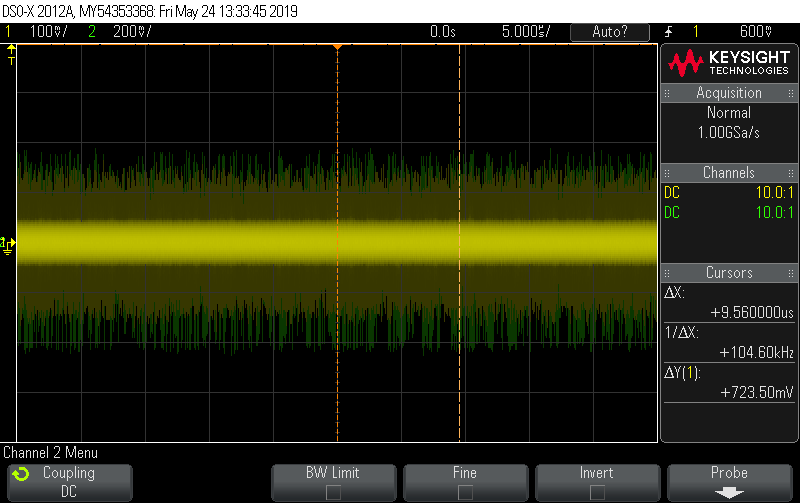
\includegraphics[width=.9\textwidth]{figures/scope_7.png}
\caption{The output voltage sampler with the input in yellow being 'FEEDBACK I/P' and the output in green being 'OP-AMP O/P'. The 'FEEDBACK I/P' is here $\approx \SI{0}{\volt}$.}
\label{fig:scope_7}
\end{figure}


\begin{figure}[H]
\centering
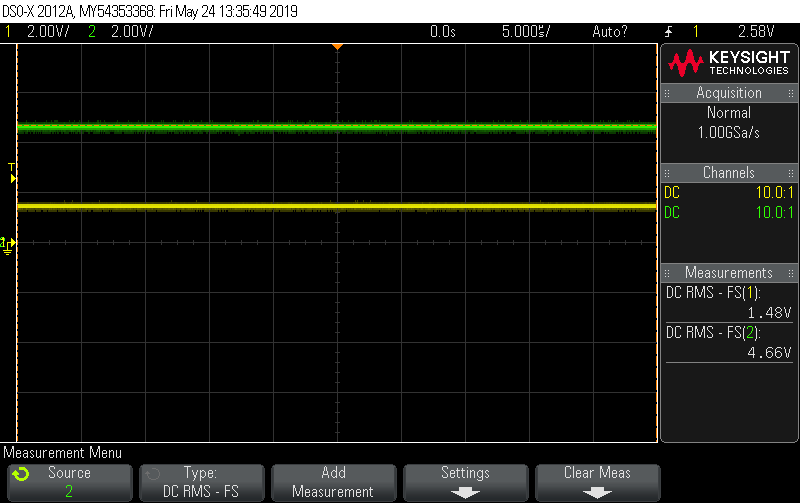
\includegraphics[width=.9\textwidth]{figures/scope_8.png}
\caption{The output voltage sampler with the input in yellow being 'FEEDBACK I/P' and the output in green being 'OP-AMP O/P'. The 'FEEDBACK I/P' is here $\approx \SI{1.5}{\volt}$.}
\label{fig:scope_8}
\end{figure}


\begin{figure}[H]
\centering
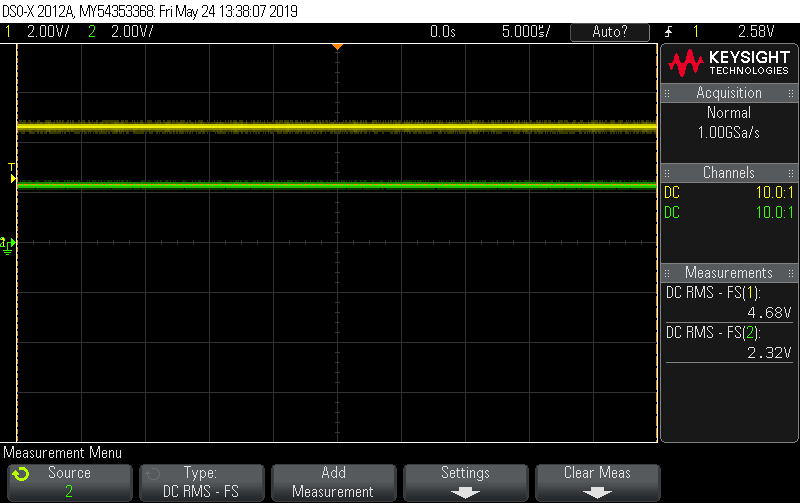
\includegraphics[width=.9\textwidth]{figures/scope_10.png}
\caption{The output voltage monitor with the input in yellow being 'OP-AMP O/P' and the output in green being 'J8 connector' or 'high voltage monitor'. The gain has been set to minimal with R16.}
\label{fig:scope_10}
\end{figure}


\begin{figure}[H]
\centering
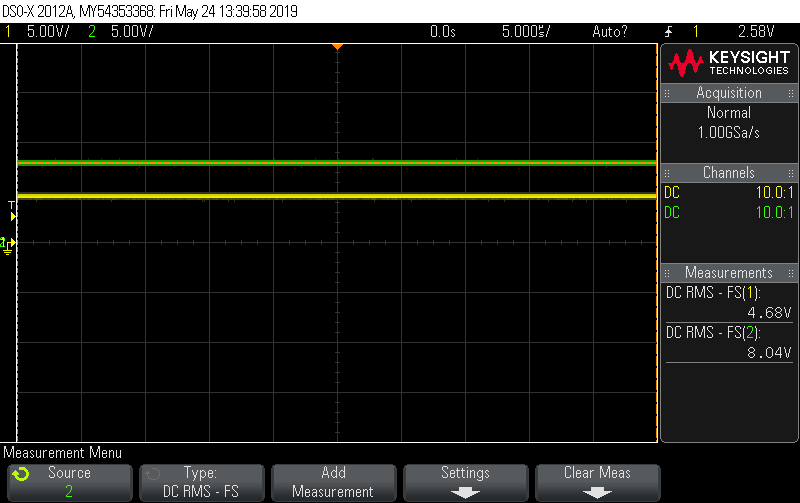
\includegraphics[width=.9\textwidth]{figures/scope_11.png}
\caption{The output voltage monitor with the input in yellow being 'OP-AMP O/P' and the output in green being 'J8 connector' or 'high voltage monitor'. The gain has been set to maximal with R16.}
\label{fig:scope_11}
\end{figure}


\begin{figure}[H]
\centering
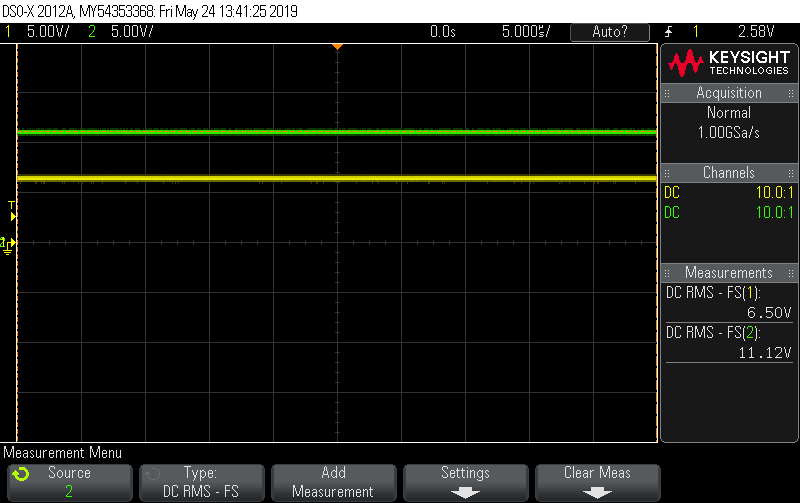
\includegraphics[width=.9\textwidth]{figures/scope_12.png}
\caption{The output voltage monitor with the input in yellow being 'OP-AMP O/P' and the output in green being 'J8 connector' or 'high voltage monitor'. The 'FEEDBACK I/P' voltage has been increased to $\SI{2}{\volt}$.}
\label{fig:scope_12}
\end{figure}

